\documentclass{article}

\usepackage{graphicx}
\usepackage{subfigure}
\usepackage[hypcap]{caption}
\usepackage{listings}
\usepackage{float}
\floatstyle{plaintop}
\restylefloat{table}

\title{Experimental Design and Data Analysis: Assignment 6}
\author{Andrew Bedard(2566978) \& Simone van Gompel(2567525) \\ Group 19}

\begin{document}

  \maketitle

  \section*{Exercise 1}
    \subsection*{1}
      This can be added to the data by using the following R-code:
      \begin{lstlisting}[language=R]
data$loglongevity = log(longevity)
      \end{lstlisting}
      Now there is a column in the data called loglongevity.

    \subsection*{2}
      In Fig\ref{fig:PairFruit} a pairplot of the fruitflies data is seen.
      Here you can see that activity and thorax have a correlation with the longevity and thus also loglongevity.
      Activity and thorax themselfs have no correlation, which is good, because that is part of the experiment set up.
      \begin{figure}[H]
          \centering
          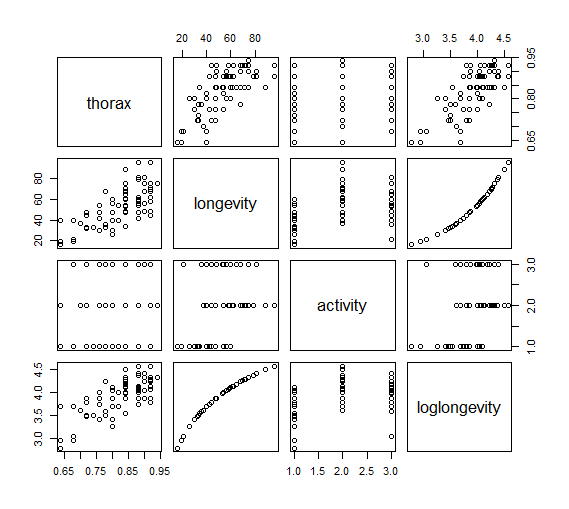
\includegraphics[scale=0.6]{../results/fruitflies2.png}
          \caption{Pairsplot Fruitflies data}
          \label{fig:PairFruit}
      \end{figure}

    \subsection*{3}
      Using anova without taking thorax length into account has $p=1.798e-07$, which means we reject $H_0$.
      This means that action has an influence on the loglongevity.

    \subsection*{4}
      In Table\ref{table:SumAction} some information can be found on the effect of action on the loglongevity.
      It is clear that the more sexual activity the fruit flies have, the shorter their lifespan was.
      The only data that does not support this is the fly that lived for the longest in low, this is higher than the rest.
      But this can be because of luck, because the mean and median are still lower than isolated.
      In Fig\ref{fig:BoxActivity} this influence is graphically shown.
      \begin{table}[H]
      \begin{center}
      \begin{tabular}{l|lll}
          \hline
                  & isolated& low & high \\
          \hline
          min     & 37      & 21  & 16 \\
          median  & 62      & 56  & 40 \\
          mean    & 63.56   & 56.76 & 38.72  \\
          max     & 75      & 81  & 60 \\
          \hline
      \end{tabular}
      \caption{Summary data of the different actions and the loglongevity}
      \label{table:SumAction}
      \end{center}
      \end{table}
      \begin{figure}[H]
          \centering
          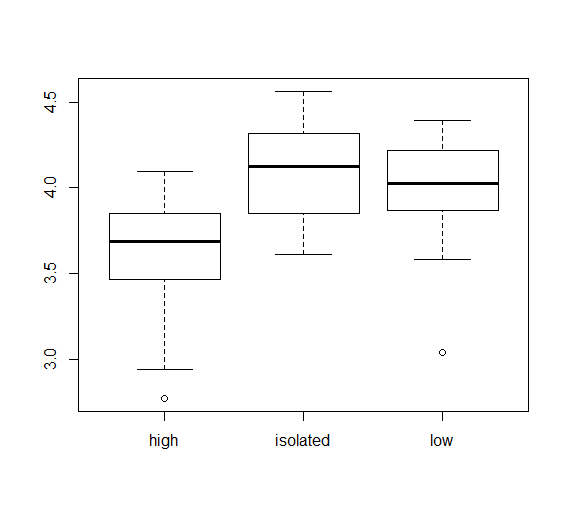
\includegraphics[scale=0.6]{../results/BoxActivity.png}
          \caption{Boxplot of the influence of activity on loglongevity}
          \label{fig:BoxActivity}
      \end{figure}

    \subsection*{5}
      Using anova, this time with taking thorax length into account has p lower than $0.05$, which means we reject $H_0$.
      This means that both action and thorax have an influence on the loglongevity.

    \subsection*{6}
      Seen in Fig\ref{fig:BoxActivity}, it is clear that sexual activity decreases the loglongevity and thus also the longevity.

    \subsection*{7}
      Thorax length increases the longevity and this stays the same over the different activities.
      The difference of the longevity between the flies with the smallest thorax and the biggest thorax are lager when there is more sexual activity.
      \begin{figure}[H]
          \centering
          \subfigure[Thorax]
          {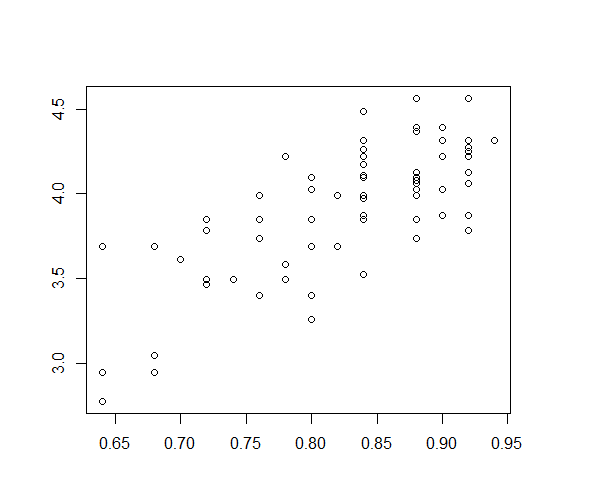
\includegraphics[scale=0.6]{../results/ScatterThorax.png}}
          \subfigure[Thorax and Activity]
          {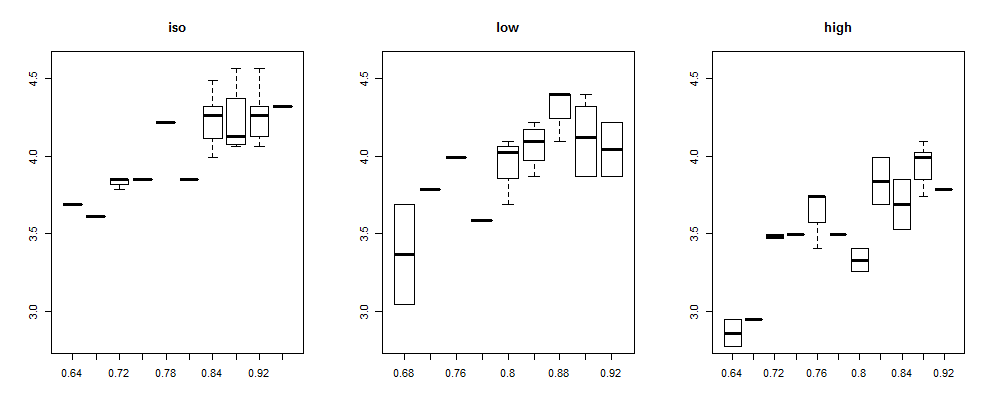
\includegraphics[scale=0.6]{../results/diffThoraxActivity.png}}
          \caption{Boxplot of the influence of activity on loglongevity}
          \label{fig:BoxActivity}
      \end{figure}

    \subsection*{8}
      My preference goes out to the analysis without thorax length, this is because the analysis of the data is harder the more variables are included. You could say the analysis with thorax length is wrong, this is not important for the research question of the data.

    \subsection*{9}
      In Fig\ref{fig:eval} the analysis that includes thorax length is evaluated.
      The qqplot shows that the residuals are normally distributed and the Fitted vs Residuals plot shows that the data has no heteroscedasticity.
      \begin{figure}[H]
          \centering
          \includegraphics[scale=0.6]{../results/evalWithThorax.png}
          \caption{Evaluation of the analysis that includes thorax length}
          \label{fig:eval}
      \end{figure}

    \subsection*{10}
      The ancova analysis with the longevity instead of the longevity has the following result:
      \begin{lstlisting}[language=R]
Response: longevity
          Df Sum Sq Mean Sq F value    Pr(>F)    
activity   2 8239.2  4119.6  38.120 5.686e-12 ***
thorax     1 7686.8  7686.8  71.127 2.624e-12 ***
Residuals 71 7673.0   108.1    
      \end{lstlisting}
      While the ancova analysis with the loglongevity had the following result:
      \begin{lstlisting}[language=R]
Response: loglongevity
          Df Sum Sq Mean Sq F value    Pr(>F)    
activity   2 3.6665  1.8332  44.606 2.838e-13 ***
thorax     1 3.8786  3.8786  94.374 1.139e-14 ***
Residuals 71 2.9180  0.0411             
      \end{lstlisting}
      This shows that with the longevity the influence of activity and thorax are bigger than with the loglongevity.
      In Fig\ref{fig:eval} the analysis of the longevity is evaluated.
      The qqplot shows that the residuals are normally distributed and the Fitted vs Residuals plot shows that the data has heteroscedasticity.
      \begin{figure}[H]
          \centering
          \includegraphics[scale=0.6]{../results/evalLongevity.png}
          \caption{Evaluation of the analysis that includes thorax length}
          \label{fig:evalLongevity}
      \end{figure}
    
  \section*{Exercise 2}
    \subsection*{1}
    The data contained in \textit{psi.txt} was read in, the following figures were obtained.
    \subsection*{2}
    Fitting a logistic regression model with psi and gpa as explanatory variables for the outcome being that the student passed their assessment or not, we obtain the following table:
    	\begin{figure}[H]
    	\begin{lstlisting}[language=R]
	Coefficients:
            Estimate Std. Error z value Pr(>|z|)   
(Intercept)  -11.602      4.213  -2.754  0.00589 **
psi            2.338      1.041   2.246  0.02470 * 
gpa            3.063      1.223   2.505  0.01224 * 
---
Signif. codes:  
0 ‘***’ 0.001 ‘**’ 0.01 ‘*’ 0.05 ‘.’ 0.1 ‘ ’ 1
    	\end{lstlisting}
    	\caption{Parameter estimation for logistic regression model}
    	\label{fig:log_reg}
    \end{figure}
    
    Thus we determine that our logistic regression model should be:
    \begin{equation}
   	Pr(\textit{pass = 1}) = \frac{\exp(-11.602 + 2.338*\textit{psi} + 3.063*\textit{gpa})}{1 + \exp(-11.602 + 2.338*\textit{psi} + 3.063*\textit{gpa})}
    \end{equation}
    \subsection*{3}
    Based on the p-value obtained in Figure:\ref{fig:log_reg}, we reject the null hypothesis that there is no effect of psi on the outcomes of the students final assessment. Further based on our parameters for the logistic regression model, we see that a positive value, ie. 1, for \textit{psi} causes an increase in probability of passing, so we conclude that \textit{psi} does in fact work.
    \subsection*{4}
    To estimate the probability that a student with a \textit{gpa} equal to 3 who receives \textit{psi} passes the assignment, we simply enter our values into equation 1, our logistic regression model.
    \[
    Pr(\textit{pass = 1}) = \frac{\exp(-11.602 + 2.338*(1) + 3.063*(3))}{1 + \exp(-11.602 + 2.338(1) + 3.063*(3))} = 0.4813
    \]
    So there is a 48.13 \% chance of a student with \textit{gpa} of 3 who receives \textit{psi} of passing the final assignment.
    
    Similarly if we wish to estimate the probability that a student with a \textit{gpa} of 3 who does not receive \textit{psi} passing the final assignment, we simply replace the value of \textit{psi} with 0, and substitute this into equation 1
    \[
    Pr(\textit{pass = 1}) = \frac{\exp(-11.602 + 2.338*(0) + 3.063*(3))}{1 + \exp(-11.602 + 2.338(0) + 3.063*(3))} = 0.0822
    \]
    Thus there is a 8.22 \% chance of a student with a \textit{gpa} of 3 who did not take \textit{psi} passing the final assignment.
    \subsection*{5}
    We may investigate the relative change in odds of passing the final assignment for students with \textit{psi} rather than those without \textit{psi} by simply taking the exponential of the change in our linear predictor, in this case taking \textit{psi} = 1 as opposed to 0 increases our linear predictor by 2.338 as we can see in Figure:\ref{fig:log_reg}, thus our difference in odds is $exp(2.338) = 10.3605$.
    
    \subsection*{6}
    Using the alternative method of analysis, and obtaining the matrix as is outlined in the R-code section \ref{sec:RE2}
        	\begin{figure}[H]
    	\begin{lstlisting}[language=R]
     [,1] [,2]
[1,]    3    8
[2,]   15    6
    	\end{lstlisting}
    \end{figure}
    Column [,1] represents students that did not receive \textit{psi}, where column [,2] are those students that did receive \textit{psi}. Row [1,] represents students that passed the final assignment, and row [2,] are those who did not pass. Thus 15 is the number of students that did not receive \textit{psi} and did not pass the final assignment, where 6 is the number of students that did receive \textit{psi} and also did not pass the final assignment.
    
    Performing the Fisher Test as outline in R-code section \ref{sec:RE2}, we obtain the following:
            	\begin{figure}[H]
    	\begin{lstlisting}[language=R]
	Fisher's Exact Test for Count Data

data:  x
p-value = 0.0265
alternative hypothesis: true odds ratio is not equal to 1
95 percent confidence interval:
 0.02016297 0.95505763
sample estimates:
odds ratio 
 0.1605805 
    	\end{lstlisting}
    \end{figure}
    The conclusion is that with a p-value of 0.0265, we should reject the null hypothesis that the probability of success for students who did and did not receive \textit{psi} is equal, thus we conclude \textit{psi} does increase a students chances of passing.
    \subsection*{7}
    
    \subsection*{8}

  \section*{Exercise 3}
    \subsection*{1}
    \subsection*{2}
    \subsection*{3}
    \subsection*{4}
    \subsection*{5}
    
  \section{R-Code}
    \subsection{Exercise 1}\label{sec:RE1}
      \begin{lstlisting}[language=R]
      \end{lstlisting}
    \subsection{Exercise 2}\label{sec:RE2}
      \begin{lstlisting}[language=R]
      \end{lstlisting}
    \subsection{Exercise 3}\label{sec:RE3}
      \begin{lstlisting}[language=R]
      \end{lstlisting}
\end{document}
